\documentclass[11pt]{article}
\usepackage[margin=1in]{geometry}
\usepackage[T1]{fontenc}
\usepackage{amsmath,amssymb,booktabs,graphicx,xcolor,array}
\usepackage[numbers,sort&compress]{natbib}
\usepackage[hidelinks]{hyperref}
\newcommand{\pending}[1]{\textcolor{red}{\textbf{PENDING}}\ (#1)}
\newcommand{\tfifty}{t_{50}}
% generated by src/build_draft.py - do not edit
\newcommand{\aucAttn}{0.786}
\newcommand{\aucDesign}{0.719}
\newcommand{\dAucAttnNoise}{+0.050}
\newcommand{\dAucAttnNoiseHi}{+0.097}
\newcommand{\dAucAttnNoiseLo}{+0.017}
\newcommand{\dAucNoiseDesign}{+0.002}
\newcommand{\devBindingBearing}{70}
\newcommand{\devScenes}{100}
\newcommand{\intAllDiff}{+0.02}
\newcommand{\intAllHi}{+0.09}
\newcommand{\intAllLo}{-0.04}
\newcommand{\pilotBindingBMN}{432}
\newcommand{\pilotBindingN}{648}
\newcommand{\pilotEligible}{0.61}
\newcommand{\pilotEligibleBM}{0.41}
\newcommand{\pilotEligibleBMN}{179}
\newcommand{\pilotEligibleN}{395}
\newcommand{\pilotFailure}{733}
\newcommand{\pilotImages}{1008}
\newcommand{\pilotPrompts}{28}
\newcommand{\pilotSeeds}{6}
\newcommand{\pilotSuccess}{275}
\newcommand{\rTwoBB}{280}
\newcommand{\rTwoBind}{0.49}
\newcommand{\rTwoChecks}{22}
\newcommand{\rTwoEligN}{113}
\newcommand{\rTwoJoint}{0.20}
\newcommand{\rTwoLatents}{2400}
\newcommand{\rTwoPassed}{22}
\newcommand{\rTwoPres}{0.40}
\newcommand{\rZeroCases}{3}
\newcommand{\rZeroHold}{all six required identities held}
\newcommand{\seedP}{0.012}
\newcommand{\testBindingBearing}{140}
\newcommand{\testScenes}{200}
\newcommand{\valAccBinding}{0.89}
\newcommand{\valAccCount}{1.00}
\newcommand{\valAccPresence}{0.93}
\newcommand{\valAccSpatial}{0.89}
\newcommand{\valNBinding}{37}
\newcommand{\valNCount}{10}
\newcommand{\valNPresence}{58}
\newcommand{\valNSpatial}{9}

\title{Guide Before Commitment: When Does a Diffusion Model Decide What It Draws, and What Does Classifier-Free Guidance Change?\\[2pt]\large Review draft: protocol, existing evidence and pending experiments}
\author{Author names and affiliations: \textit{placeholder}}
\date{Draft generated from verified artifacts; see \texttt{docs/RESULTS\_PROVENANCE.md}}
\begin{document}
\maketitle
\begin{abstract}
Text-to-image diffusion models often produce plausible images that violate parts of the prompt: an object is missing, a colour lands on the wrong object, a count, a relative size or a spatial relation is wrong.
We study \emph{when} each of these constraints becomes stable during denoising and \emph{what classifier-free guidance (CFG) changes about it}, on Stable Diffusion~1.5 and a controlled scene-graph benchmark with a factorial family built around the problem statement's example (``a small red cube and a large blue sphere'').
Two interventional probes estimate a chance-corrected restart-persistence step $t_{50}$ per constraint type: re-noising a saved trajectory state and switching from a counterfactual to the canonical prompt mid-trajectory.
Four pre-specified hypotheses ask whether $t_{50}$ differs between constraint types (HA), whether higher CFG moves it earlier (HD), whether the step at which cross-attention stops changing tracks it without labels (HF), and whether a guidance schedule that switches from high to low guidance after the DEV-measured step keeps adherence while raising seed diversity and beating a reversed schedule (HE).
This draft reports only what exists: an exploratory 28-prompt pilot, reproducibility and integrity checks of the first Kaggle runs, and a first-pass, still unaudited, evaluation of \rTwoBB{} development images. \textbf{All confirmatory results are pending}; the test split is sealed and the protocol is not frozen.
\end{abstract}

\section{Introduction}
Prompt adherence of text-to-image diffusion models is usually summarised by one score per image. Compositional failures, however, are constraint-specific: an object can be present while its colour is wrong, or two objects can be correct while their left--right order is not. If different constraints are resolved at different moments of the sampling trajectory, three practical consequences follow. Guidance strength that matters early may be wasted late; diagnostics that read early internal signals are forecasts for some constraints and read-outs for others; and a pooled adherence score can hide both effects.

Prior work establishes that denoising stages control different image properties \citep{patashnik2023mixing,zhang2023prospect,balaji2022ediffi,li2024critical}, that guidance can be restricted or scheduled over time \citep{kynkaanniemi2024interval,sadat2024cads,dynamiccfg2025}, and that cross-attention carries information about objects and attributes that can be read and steered \citep{hertz2023p2p,tang2023daam,chefer2023attend,epstein2023selfguidance}. We therefore do not claim that the general idea of stage-dependent generation is new. Our questions are narrower and measurement-first:
\begin{enumerate}
\item \textbf{When} does each constraint type (presence, count, colour binding, spatial relation, relative size) stop depending on the remaining randomness of the trajectory? We answer with an interventional, chance-corrected persistence curve rather than with an observational signal.
\item \textbf{What does CFG change?} Does a larger guidance scale move persistence earlier, once the higher seed-to-seed agreement it induces is accounted for?
\item \textbf{Can attention tell?} Does the step at which cross-attention stops changing track the interventional measurement?
\item \textbf{Is the timing usable?} Does a two-level guidance schedule whose switch step is read off development-set measurements keep adherence while raising diversity, and does it beat the same mean guidance applied in reverse order?
\end{enumerate}

\paragraph{Contributions.}
\begin{enumerate}
\item[(i)] An interventional, chance-corrected measurement of restart persistence per constraint type, with two re-noising probes and a closed-form stress test for judge error (Section~\ref{sec:methods}).
\item[(ii)] A controlled scene-graph benchmark with counterfactual variants and a factorial size family, scored by a judge whose blinded human audit decides which constraint types may carry claims (Sections~\ref{sec:benchmark}--\ref{sec:evaluation}).
\item[(iii)] Commitment-Aligned Guidance (CAG), tested against constant, reversed and matched-mean schedules under a signed pre-registration, with every gate reported whether it passed or failed (Sections~\ref{sec:methods} and~\ref{sec:resDEV}).
\item[(iv)] On the available test shards, an account of what survives: the guidance effect on timing, its sensitivity to the judge, the failure of commitment times to transfer, the dose explanation of CAG's diversity gain, and what saved cross-attention maps add to the restart measurement (Sections~\ref{sec:resPARTIAL}--\ref{sec:resATTN}).
\end{enumerate}

\paragraph{Findings in brief (partial test split, exploratory).}
\begin{itemize}
\item Stronger guidance makes object presence persistent earlier, with $t_{50}(w{=}15)-t_{50}(w{=}2)=\rbHdReg$ of 40 steps. This is the only registered rule that passed. The effect is not an artefact of the chance correction or of the full-resample offset. It does assume that the presence judge's errors are not independent across seeds.
\item Cross-attention moves in the same direction: higher guidance separates the object nouns and makes their attention stabilise earlier. Objects that are eventually missed have diffuse, overlapping attention from the first steps.
\item Attention stabilisation does not order the constraint types the way persistence does. Its binding signal follows object layout, not colour assignment.
\item Commitment times measured on the development split did not transfer to the test scenes, so CAG switched guidance down before binding had settled. CAG was not non-inferior to constant guidance, and its diversity gain is explained by its lower mean guidance.
\end{itemize}
We use the operational term \emph{restart persistence}; we do not claim that the model ``decides'' in any cognitive sense. Figure~\ref{fig:concept} summarises the probes and the schedule.
\begin{figure}[t]\centering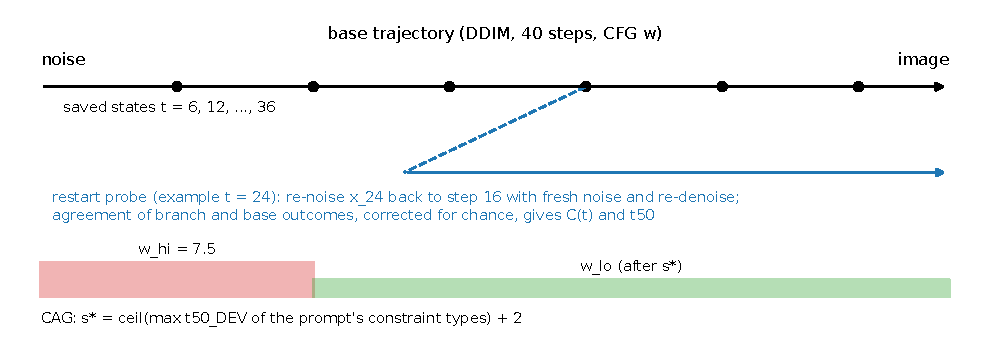
\includegraphics[width=\linewidth]{figures/fig_concept.pdf}
\caption{\textbf{Conceptual diagram} (not data). Top: a 40-step DDIM trajectory with saved states. Middle: the restart probe re-noises a saved state to an earlier step with fresh noise and re-denoises; agreement of branch and base outcomes, corrected for chance agreement between independent seeds, gives $C(t)$ and $t_{50}$. Bottom: CAG applies $w_{hi}$ until a prompt-specific switch step $s^\star$ derived from development-set $t_{50}$, then $w_{lo}$.}\label{fig:concept}\end{figure}

\section{Related work}\label{sec:related}
\paragraph{Diffusion sampling and guidance.} We use denoising diffusion models \citep{ho2020ddpm}, deterministic DDIM sampling \citep{song2021ddim}, latent diffusion \citep{rombach2022ldm} and classifier-free guidance \citep{ho2022cfg}. Restricting guidance to an interval of noise levels has been reported to improve sample quality \citep{kynkaanniemi2024interval}, annealing the conditioning signal early to restore diversity \citep{sadat2024cads}, and choosing per-step guidance online with latent evaluators to be prompt-dependent \citep{dynamiccfg2025}. Add-noise-then-denoise operations are used for editing and for sampling \citep{meng2022sdedit,xu2023restart}; we use re-noising only as a \emph{measurement}.

\paragraph{Stages of generation.} Switching prompts over denoising intervals localises layout, shape and detail to successive stages \citep{patashnik2023mixing}; stage-specific text embeddings control different attributes \citep{zhang2023prospect}; an ensemble of stage-specialised denoisers is motivated by text conditioning mattering most early \citep{balaji2022ediffi}; and features have been analysed theoretically as emerging in narrow time windows \citep{li2024critical}. Strengthening the conditioning signal at selected steps has been reported to improve alignment more when done late than early \citep{grimal2025step}, a finding in tension with front-loading guidance, and negative prompts to act with a delay \citep{ban2024negative}.

\paragraph{Cross-attention.} Cross-attention maps are used to interpret \citep{tang2023daam} and edit \citep{hertz2023p2p} generations, and attention-based objectives target object neglect and attribute binding \citep{chefer2023attend,li2023divide,fu2024gather,rassin2023syngen}; attention can also read and steer object size and position \citep{epstein2023selfguidance}. Initial-noise search and early prediction of image quality from attention are close in aim to our attention analysis \citep{guo2024initno,diffusionprobe2026}.

\paragraph{Evaluation.} Object-focused and question-answering evaluators \citep{ghosh2023geneval,huang2023t2icompbench,hu2023tifa,kamath2025geneval2} motivate our emphasis on judge reliability. Our judge combines open-vocabulary detection \citep{minderer2022owlvit} with CLIP \citep{radford2021clip}; seed diversity uses DINOv2 embeddings \citep{oquab2024dinov2}.

\paragraph{Position of this work.} Table~\ref{tab:related} contrasts what the closest methods measure, intervene on and evaluate. The common thread is that timing matters; the differences are that we (a) measure timing \emph{interventionally and per constraint type} with an explicit chance correction, (b) test whether CFG moves that timing, (c) compare an unsupervised attention signal against the interventional one, and (d) derive a guidance switch from the measurement rather than tuning it on adherence. To our knowledge these four elements have not been combined on controlled scene graphs; the literature search was narrow (Table~\ref{tab:related} caption) and this is a candidate gap, not an established one.
\begin{table*}[t]\centering\small
\caption{Closest prior work and this study: what each method measures, what it changes during sampling, and how it is evaluated. ``--'': not an aim of the method. Descriptions of Prompt-to-Prompt and Attend-and-Excite were checked against the full papers, the others against their abstracts (marked in the bibliography source).}\label{tab:related}
\begin{tabular}{p{2.9cm}p{3.7cm}p{3.7cm}p{3.7cm}}
\toprule
Method & Measures & Intervenes on & Evaluated by \\
\midrule
Prompt-to-Prompt \citep{hertz2023p2p} & -- & cross-attention maps (injection, re-weighting) to edit an image & edit fidelity, qualitative and quantitative \\
Attend-and-Excite \citep{chefer2023attend} & subject-token attention as a neglect signal & latents at inference, to raise neglected tokens' attention & object presence and binding (CLIP-based metrics, user study) \\
Prompt Mixing \citep{patashnik2023mixing} & -- & which prompt is used in which denoising interval & localisation of shape variations \\
Critical windows \citep{li2024critical} & time windows in which features emerge (theory) & -- & theory and experiments \\
Interval guidance \citep{kynkaanniemi2024interval} & -- & CFG applied only in a limited noise interval & distribution and sample quality \\
CADS \citep{sadat2024cads} & -- & conditioning annealed with noise early in sampling & diversity and quality \\
Dynamic CFG \citep{dynamiccfg2025} & per-step feedback from latent evaluators & per-step guidance scale, chosen online & prompt adherence and quality \\
Step selection \citep{grimal2025step} & -- & conditioning signal strengthened at selected steps & text--image alignment \\
InitNO \citep{guo2024initno} & attention-based validity of the initial noise & initial noise, optimised before sampling & text--image alignment \\
Diffusion Probe \citep{diffusionprobe2026} & early cross-attention as a predictor of final quality & -- (used for prompt and seed selection) & prediction accuracy \\
\midrule
This study & interventional, chance-corrected persistence $C(t)$ and $t_{50}$ per constraint type; attention stabilisation & two-level CFG switched at a step derived from development-set $t_{50}$ (CAG) & pre-registered tests with a human-audited judge; constant, reversed and matched-mean schedule controls \\
\bottomrule
\end{tabular}
\end{table*}


\section{Research questions and hypotheses}\label{sec:rq}
The four confirmatory hypotheses form one Holm family ($\alpha=0.05$); a hypothesis is reported as supported only if its own decision rule passes and its Holm-adjusted $p<0.05$. The definitions below are copied from the draft Addendum~C, which is \textbf{not frozen}.

\paragraph{HA, constraint-specific persistence.} Primary estimand $\Delta t_{50}=t_{50}^{\mathrm{bind\mid pres}}-t_{50}^{\mathrm{presence}}$ at $w=7.5$. Support: the 95\% scene-bootstrap interval excludes $0$, $|\Delta t_{50}|\ge3$ steps, the joint companion and the equal-ratio restart agree in sign. Bounded null: interval inside $(-1.5,1.5)$. The predicted ordering is presence $\approx$ size $<$ spatial $<$ colour binding; the position of count is declared exploratory.
\paragraph{HD, CFG moves persistence.} $t_{50}(w=15)-t_{50}(w=2)$ for presence and for binding given presence, with the chance level $A0$ computed at each $w$ and one shared resample of scenes; supported if at least one estimand is negative with $|\Delta|\ge3$ and the interval excludes $0$ ($p_{HD}=\min(1,2\min p)$); a positive interval is reported as contradicted.
\paragraph{HF, attention stabilisation.} The step at which half of the attention signal's path length has been travelled ($t_{\mathrm{stab}}$) per constraint type; support if the ordering concordance with $t_{50}$ is at least $0.8$ and the within-type Spearman correlation between scene $t_{\mathrm{stab}}$ and the scene's area under the commitment curve has an interval above $0$ for at least two types.
\paragraph{HE, Commitment-Aligned Guidance.} $s^\star=\lceil\max_{\kappa}t_{50,\mathrm{DEV}}^{\kappa}\rceil+2$ over the prompt's constraint types; $w=7.5$ before $s^\star$, $w=1$ after. Supported only if, jointly, adherence is non-inferior to constant CFG~7.5 (90\% interval lower bound above $-0.03$), seed diversity is higher (95\% interval above $0$), and CAG beats the reversed schedule with equal mean guidance (95\% interval above $0$).
\begin{table}[t]
\centering\small
\caption{Status of the four confirmatory hypotheses (Revision 3). No confirmatory data exist.}
\label{tab:hypotheses}
\begin{tabular}{llp{6.2cm}}
\toprule
ID & Question & Status \\
\midrule
HA & Restart persistence differs between constraint types (presence, count, size, spatial, colour binding) & \textbf{PENDING}: DEV/TEST restart branches not run; DEV gate not evaluated; TEST sealed \\
HD & Higher CFG moves the restart-persistence step earlier & \textbf{PENDING}: needs TEST branches at CFG 2 / 7.5 / 15; TEST sealed \\
HE & Commitment-Aligned Guidance: non-inferior adherence, higher diversity, beats the reversed schedule & \textbf{PENDING}: needs DEV-derived switch steps, quality-guard decision and TEST arms \\
HF & Attention stabilisation tracks restart persistence & \textbf{PENDING}: needs TEST attention maps and HA curves \\
\bottomrule
\end{tabular}
\end{table}


\section{Methods}\label{sec:methods}
\paragraph{Generator.} Stable Diffusion~1.5 \citep{rombach2022ldm} at a pinned revision in fp16, DDIM \citep{song2021ddim} with $\eta=0$ and $T=40$ steps at $512^2$ pixels, empty negative prompt. With text condition $c$ and guidance scale $w$, the noise prediction at step $i$ is the classifier-free combination \citep{ho2022cfg}
\begin{equation}
\hat\varepsilon_i = \varepsilon_\theta(x_i,\varnothing) + w_i\,\big(\varepsilon_\theta(x_i,c)-\varepsilon_\theta(x_i,\varnothing)\big),
\end{equation}
where $w_i$ is constant ($w_i=w$) except under the guidance schedules below. When $w_i=1$ only the conditional branch is evaluated, and the number of network evaluations is counted per image.

\paragraph{Outcomes.} An automatic judge (Section~\ref{sec:evaluation}) scores each image for each constraint $\kappa$ of its prompt: presence (all required objects detected), count (exact), and, conditional on the relevant objects being present, colour binding, left/right relation and relative size (box area of the intended larger object at least $1.5\times$ the other's). Conditional outcomes are undefined, not zero, when an object is missing. The adherence score $F$ of an image is the mean of the outcome families present.

\paragraph{Restart probe.} The latent after $t\in\mathcal{G}=\{6,12,18,24,30,36\}$ completed steps is saved. A branch re-noises it to an earlier step index $j$ with fresh noise $\varepsilon\sim\mathcal{N}(0,I)$ and denoises deterministically to the end at the base's guidance:
\begin{equation}
x'_j=\sqrt{r}\,x_t+\sqrt{1-r}\,\varepsilon,\qquad r=\bar\alpha(j)/\bar\alpha(t),
\end{equation}
with $\bar\alpha(s)$ taken at the scheduler timestep of step $s$. The fixed-jump probe (D8) uses $j=\max(t-8,0)$, whose noise share $1-r$ grows with $t$; the equal-ratio probe (ER30) chooses $j$ so that $r\approx0.30$ at every $t$; a full resample (FULL) restarts from pure noise and serves as a validity control.

\paragraph{Chance-corrected persistence.} For scene $s$ and constraint type $\kappa$, let $A_{\kappa s}(t)$ be the share of (base, branch) pairs with equal outcomes and $A0_{\kappa s}$ the agreement between independent seeds of the \emph{same base prompt, guidance and step count}. Persistence pools scenes as a ratio estimator,
\begin{equation}
C_\kappa(t)=\frac{\sum_s\big[A_{\kappa s}(t)-A0_{\kappa s}\big]}{\sum_s\big[1-A0_{\kappa s}\big]},
\end{equation}
so $C=0$ means no more agreement than an independent sample and $C=1$ means the outcome is fixed. $t_{50}^\kappa$ is the linearly interpolated first crossing of $0.5$; it is left-censored when $C$ already exceeds $0.5$ at $t=6$ and right-censored when it never does. Because the noise share of D8 varies with $t$, absolute $t_{50}$ is relative to the probe; ER30 is the registered sensitivity check.

\paragraph{Prompt-switch probe.} A counterfactual trajectory (colour swap, relation reversal or size swap) is continued from its saved state with the canonical prompt, and
\begin{equation}
C^{\mathrm{switch}}(t)=\frac{\sum_s\big[W_s(t)-W0_s\big]}{\sum_s\big[W1_s-W0_s\big]},
\end{equation}
where $W$ is the share of switched images satisfying the counterfactual constraint and $W0$, $W1$ are that share among canonical and counterfactual images.

\paragraph{Attention stabilisation.} Cross-attention maps of the constraint words are recorded at every step (conditional branch, averaged over heads and over layers within the $16\times16$ and $32\times32$ groups; recording leaves the image unchanged). Per type a signal $a_i$ is formed (noun map, colour-word map, ratio of effective areas, angle between noun centroids, connected components), its velocity $v_i=1-\cos(a_i,a_{i-1})$ (or the absolute change of a scalar), and $t_{\mathrm{stab}}$ is the step at which half of the cumulative path $\sum_i v_i$ has been travelled.

\paragraph{Commitment-Aligned Guidance.} For a prompt with constraint types $K$, the switch step and the schedules are
\begin{equation}
s^\star=\min\!\Big(\big\lceil\max_{\kappa\in K}t_{50,\mathrm{DEV}}^{\kappa}\big\rceil+2,\;T\Big),\qquad
w_i^{\mathrm{A2}}=\begin{cases}w_{hi}&i<s^\star\\ w_{lo}&i\ge s^\star\end{cases},\qquad
w_i^{\mathrm{A4}}=\begin{cases}w_{lo}&i<s^\star\\ w_{lo}+\frac{s^\star(w_{hi}-w_{lo})}{T-s^\star}&i\ge s^\star\end{cases},
\end{equation}
with $w_{hi}=7.5$. A4 has the same mean guidance as A2 in reverse order; A6 applies that mean as a constant; A3 uses a global $s^\star$ from the median DEV $t_{50}$; A1 is constant $7.5$. The frozen design uses $w_{lo}=\wLo$, selected by the DEV quality guard (Section~\ref{sec:resDEV}); Figure~\ref{fig:schedules} shows the exact schedules for the two switch steps that occur on the test split.
\begin{figure}[t]\centering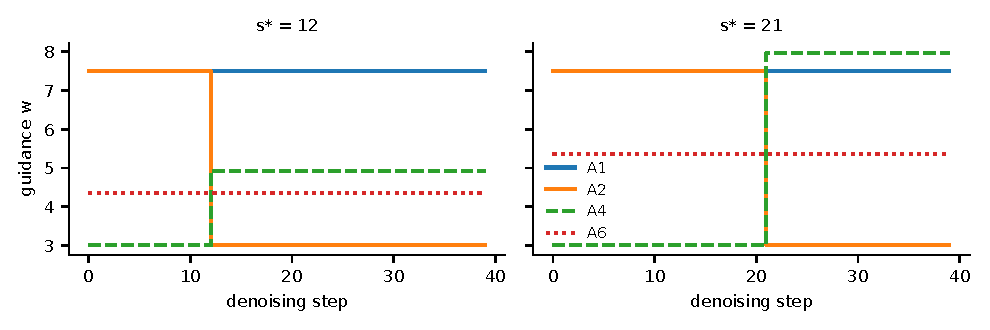
\includegraphics[width=\linewidth]{figures/fig_cag_schedules.pdf}
\caption{Exact guidance schedules of the frozen design (computed by \texttt{src/cag.py}) for $s^\star=12$ and $s^\star=21$ with $w_{lo}=\wLo$: constant CFG (A1), CAG (A2), reversed with equal mean (A4) and constant at A2's mean (A6). A4 is not capped; its maximum guidance is recorded per job.}\label{fig:schedules}\end{figure}

\paragraph{Statistical analysis.} Uncertainty uses a scene-level bootstrap with $10{,}000$ draws and fixed random keys, resampling scenes (not images) so that seeds and branches of a scene stay together; $p$-values are bootstrap tail probabilities. Holm's procedure controls the family-wise error over HA, HD, HE and HF, with a non-estimable hypothesis counting as $p=1$. Identical generations (same prompt text, guidance, steps and seed in one split) are counted once, two canonical scenes with identical text count once, and test prompts whose text also occurs in the development split are excluded from variant-level summaries.

\paragraph{Sensitivity to judge error (exploratory, not registered).} Restart persistence is a statement about agreement between judged outcomes, so judge errors enter both $A$ and $A0$. If each judged outcome is flipped independently with probability $e$ (symmetric, non-differential error), every observed agreement is the affine image $A^{\mathrm{obs}}=(1-2e)^2A+c$ of the true agreement with $c=2e(1-e)$, for branch pairs and seed pairs alike. Substituting into the pooled estimator gives the error-corrected persistence
\begin{equation}\label{eq:err-corr}
C_\kappa^{(e)}(t)=\frac{\sum_s\big[A^{\mathrm{obs}}_{\kappa s}(t)-A0^{\mathrm{obs}}_{\kappa s}\big]}{\sum_s\big[1-c-A0^{\mathrm{obs}}_{\kappa s}\big]},
\end{equation}
which equals the registered $C_\kappa(t)$ at $e=0$. Error makes $C$ shrink towards zero by an amount that depends on $A0$, which differs between guidance scales. The model assumes errors independent across images; a detector's errors are usually content-dependent (the same hard object is missed in every seed), which can move agreement in either direction and is not captured. We therefore use Eq.~\eqref{eq:err-corr} as a stress test of how much judge noise a conclusion tolerates, not as a correction of the estimate, and evaluate $e\in\{0.05,0.10\}$ and $e=1-\text{(audited presence accuracy)}$.

\section{Benchmark V2}\label{sec:benchmark}
Prompts are generated from machine-readable scene graphs with a grammar and lexicon; every scene has a canonical prompt and meaning-preserving and counterfactual variants (each counterfactual changes exactly one declared field), split at scene level with object-pair groups confined to one split. The main benchmark has \devScenes{} DEV and \testScenes{} TEST scenes; because some variant types are inapplicable to some scene types it contains 1,410 prompts rather than the 1,500 of the design. A separate factorial family of 24 object pairs (8 DEV, 16 TEST) crosses colour, relative size and spatial relation on top of presence (192 canonical prompts plus colour-swap, size-swap and relation-reversal counterfactuals). Human review of variants and the lexicon freeze are \textbf{pending}.
\begin{table}[t]
\centering\small
\caption{Benchmark V2 design counts (scene graphs are the independent unit). TEST counts are design counts; the generated TEST shards are listed in Table~\ref{tab:partial-cov}.}
\label{tab:benchmark}
\begin{tabular}{lrrrrr}
\toprule
Split & Scenes & Binding-bearing (literal) & Competitive subset & Spatial-bearing & Prompt variants \\
\midrule
DEV & 100 & 70 & 55 & 28 & 470 \\
TEST & 200 & 140 & 110 & 54 & 940 \\
\bottomrule
\end{tabular}
\end{table}


\section{Evaluation and judge audit}\label{sec:evaluation}
The judge (J1) combines open-vocabulary detection \citep{minderer2022owlvit} with CLIP colour classification \citep{radford2021clip} at pinned model revisions, with thresholds fixed before any test data (presence 0.10, count 0.15, size ratio 1.5). A second, question-answering judge was planned but not implemented and plays no role in any result.

\paragraph{Pre-declared audit.} A blinded, seeded, stratified sample of DEV (image, constraint) items was labelled by a human who saw only an opaque image and a neutral question (a colour, a count, a presence answer, which object is further left, or which looks larger), with ``not visible'' and ``ambiguous'' answers. Accuracy is population-weighted with a stratified bootstrap. A constraint type may carry a confirmatory claim only if its weighted accuracy is at least $0.85$; no other criterion was added after the data were seen.

\paragraph{Result.} Only presence met the criterion (Table~\ref{tab:dev-audit}, Figure~\ref{fig:audit}). The binding judge reached \accBind, count \accCount, spatial relation \accSpat{} (its sensitivity was low) and relative size \accSize. One annotator labelled the main package; a second package was labelled by the same person within the same session and is therefore neither an inter-rater nor a valid intra-rater check, and is not used. These limits are carried into every result (Section~\ref{sec:rq}).
% generated by paper/make_paper_assets.py from docs/evidence/audit_20261019/audit_verdicts.json
\begin{table}[t]
\centering\small
\caption{DEV evaluator audit of J1 against blinded human labels (one annotator; population-weighted accuracy, stratified bootstrap 95\% CI). Only types meeting $\geq 0.85$ may carry a confirmatory claim.}
\label{tab:dev-audit}
\begin{tabular}{lrrrr}
\toprule
Type & $n$ & Accuracy & 95\% CI & $\geq 0.85$ \\
\midrule
presence & 159 & 0.856 & [0.802, 0.907] & yes \\
count & 108 & 0.768 & [0.685, 0.843] & no \\
binding & 156 & 0.800 & [0.722, 0.871] & no \\
spatial & 109 & 0.615 & [0.523, 0.706] & no \\
size & 175 & 0.846 & [0.794, 0.897] & no \\
\bottomrule
\end{tabular}
\end{table}

\begin{figure}[t]\centering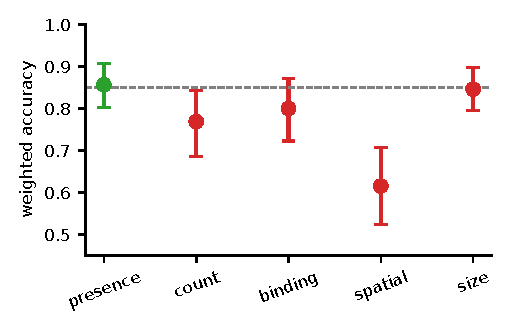
\includegraphics[width=0.55\linewidth]{figures/fig_audit.pdf}
\caption{Weighted accuracy of the automatic judge per constraint type on DEV (95\% bootstrap intervals; one annotator). Dashed line: pre-declared criterion $0.85$. Green: met; red: not met.}\label{fig:audit}\end{figure}

\section{Experimental design and execution}\label{sec:design}
All jobs come from deterministic manifests sharded by scene group over three workers (Table~\ref{tab:design}). A stage guard refuses any stage whose owner-controlled gates are false, and test jobs are refused unless the signed protocol verifies against the code, configurations, benchmark, judge definition and development-set constants. Every worker output is merged against its manifest before analysis; missing, duplicated, corrupt or mismatching outputs are rejected, never silently dropped.
The development stages ran first: the canonical DEV core (400 images: 100 prompts, four seeds, saved states; restarts branch from seeds 0 and 1), the DEV variants and size family (\devCoreJobs{} jobs), restart branches and CFG bases (\devCommitJobs{} jobs) and the CAG quality guard (\devCagJobs{} jobs). The test split comprises \testCoreJobs{} core and CFG$\times$steps jobs, \testCommitJobs{} restart and switch jobs, and \testCagJobs{} CAG and size-family jobs (\testEq{} full-generation equivalents). Generation used two NVIDIA T4 GPUs at about 7.0~s per 40-step image per GPU.
\begin{table}[t]\centering\small
\caption{Frozen stage manifests (job counts and full-generation equivalents from \texttt{src/manifests.py} with the frozen constants).}\label{tab:design}
\begin{tabular}{llp{6.3cm}rr}
\toprule
Split & Stage & Content & Jobs & Equiv. \\
\midrule
DEV & DEV\_CORE & variants, CF bases, DEV size family & 1,784 & 1,784 \\
DEV & DEV\_COMMIT & restarts D8/ER30/FULL, CFG 2/15 bases and restarts, switches & 8,896 & 6,930 \\
DEV & DEV\_CAG\_GUARD & CAG $w_{lo}\in\{1,3\}$ quality guard & 400 & 336 \\
TEST & TEST\_CORE & all variants; CFG $\times$ steps & 9,160 & 7,660 \\
TEST & TEST\_COMMIT & restarts at CFG 2/7.5/15; prompt switches & 10,560 & 6,986 \\
TEST & TEST\_CAG\_SIZE & CAG arms A2/A3/A4/A6; size family with restarts and switches & 5,536 & 4,923 \\
\bottomrule
\end{tabular}
\end{table}


\section{Earlier evidence: pilot and infrastructure (exploratory)}\label{sec:existing}
This section reports the pilot that motivated the study, (A), the infrastructure and integrity checks of the first cloud runs, (B), and a first-pass look at the DEV core made before the judge audit, (C). None of it tests the registered hypotheses.

\subsection{A. Pilot (exploratory)}
The pilot generated \pilotImages{} images (\pilotPrompts{} prompts, three CFG scales, two step counts, \pilotSeeds{} seeds). Table~\ref{tab:pilot-adherence} and Figure~\ref{fig:pilot} show constraint satisfaction; CFG contrasts are in Table~\ref{tab:pilot-cfg}. With only $4$--$6$ prompts per category the intervals are wide and no CFG effect on adherence is resolved; absence of a resolved effect is not evidence of its absence.
\begin{figure}[t]\centering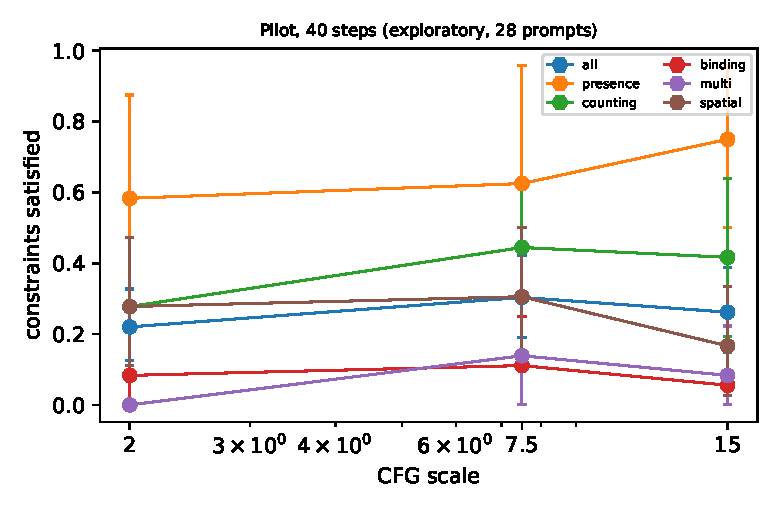
\includegraphics[width=0.7\linewidth]{figures/pilot_adherence.pdf}\caption{Pilot constraint satisfaction against CFG (40 steps, exploratory).}\label{fig:pilot}\end{figure}
\begin{table}[t]
\centering\small
\caption{Pilot (28 prompts, detector-based labels, exploratory): fraction of constraints satisfied, by category, CFG and inference steps; 95\% prompt-cluster bootstrap intervals.}
\label{tab:pilot-adherence}
\begin{tabular}{llrrr}
\toprule
Category & CFG & 20 steps & 40 steps & Prompts \\
\midrule
all & 2 & 0.24 [0.137, 0.351] & 0.22 [0.125, 0.327] & 28 \\
all & 7.5 & 0.30 [0.190, 0.417] & 0.30 [0.190, 0.423] & 28 \\
all & 15 & 0.32 [0.202, 0.440] & 0.26 [0.149, 0.387] & 28 \\
presence & 2 & 0.58 [0.292, 0.875] & 0.58 [0.292, 0.875] & 4 \\
presence & 7.5 & 0.71 [0.417, 0.958] & 0.62 [0.292, 0.958] & 4 \\
presence & 15 & 0.67 [0.292, 1.000] & 0.75 [0.500, 0.958] & 4 \\
counting & 2 & 0.36 [0.167, 0.583] & 0.28 [0.111, 0.472] & 6 \\
counting & 7.5 & 0.39 [0.194, 0.611] & 0.44 [0.250, 0.639] & 6 \\
counting & 15 & 0.44 [0.250, 0.639] & 0.42 [0.194, 0.639] & 6 \\
binding & 2 & 0.06 [0.000, 0.194] & 0.08 [0.000, 0.222] & 6 \\
binding & 7.5 & 0.11 [0.000, 0.278] & 0.11 [0.000, 0.250] & 6 \\
binding & 15 & 0.17 [0.028, 0.333] & 0.06 [0.000, 0.167] & 6 \\
multi & 2 & 0.00 [0.000, 0.000] & 0.00 [0.000, 0.000] & 6 \\
multi & 7.5 & 0.11 [0.000, 0.333] & 0.14 [0.000, 0.306] & 6 \\
multi & 15 & 0.08 [0.000, 0.250] & 0.08 [0.000, 0.223] & 6 \\
spatial & 2 & 0.31 [0.111, 0.500] & 0.28 [0.111, 0.472] & 6 \\
spatial & 7.5 & 0.31 [0.139, 0.500] & 0.31 [0.111, 0.500] & 6 \\
spatial & 15 & 0.33 [0.167, 0.528] & 0.17 [0.028, 0.333] & 6 \\
\bottomrule
\end{tabular}
\par\smallskip\footnotesize Intervals resample prompts; the judge is unaudited on the DEV set.
\end{table}

\begin{table}[t]
\centering\small
\caption{Pilot CFG contrasts (paired by prompt and seed; Holm-adjusted $p$ from Wilcoxon tests), exploratory.}
\label{tab:pilot-cfg}
\begin{tabular}{llrrrr}
\toprule
Category & CFG a vs b & Diff. & 95\% CI & Prompts & $p_{Holm}$ \\
\midrule
presence & 2 vs 7.5 & -0.083 & [-0.438, 0.229] & 4 & 1.000 \\
presence & 2 vs 15 & -0.125 & [-0.500, 0.250] & 4 & 1.000 \\
presence & 7.5 vs 15 & -0.042 & [-0.208, 0.104] & 4 & 1.000 \\
binding & 2 vs 7.5 & -0.042 & [-0.181, 0.097] & 6 & 1.000 \\
binding & 2 vs 15 & -0.042 & [-0.153, 0.083] & 6 & 1.000 \\
binding & 7.5 vs 15 & +0.000 & [-0.111, 0.125] & 6 & 1.000 \\
counting & 2 vs 7.5 & -0.097 & [-0.292, 0.083] & 6 & 1.000 \\
counting & 2 vs 15 & -0.111 & [-0.333, 0.083] & 6 & 1.000 \\
counting & 7.5 vs 15 & -0.014 & [-0.097, 0.056] & 6 & 1.000 \\
spatial & 2 vs 7.5 & -0.014 & [-0.167, 0.153] & 6 & 1.000 \\
spatial & 2 vs 15 & +0.042 & [-0.069, 0.125] & 6 & 0.750 \\
spatial & 7.5 vs 15 & +0.056 & [-0.069, 0.181] & 6 & 1.000 \\
multi & 2 vs 7.5 & -0.125 & [-0.292, 0.000] & 6 & 0.750 \\
multi & 2 vs 15 & -0.083 & [-0.222, 0.000] & 6 & 1.000 \\
multi & 7.5 vs 15 & +0.042 & [-0.083, 0.208] & 6 & 1.000 \\
all & 2 vs 7.5 & -0.071 & [-0.155, 0.009] & 28 & 0.174 \\
all & 2 vs 15 & -0.060 & [-0.146, 0.018] & 28 & 0.214 \\
all & 7.5 vs 15 & +0.012 & [-0.045, 0.071] & 28 & 0.873 \\
\bottomrule
\end{tabular}
\end{table}

Global attention re-weighting (scale~2 against the control path) changed overall adherence by \intAllDiff{} (95\% CI \intAllLo{} to \intAllHi{}), i.e.\ no resolved improvement (Table~\ref{tab:pilot-intervention}).
\begin{table}[t]
\centering\small
\caption{Pilot global attention re-weighting (scale 2 and 4 against the scale-1 control path), primary outcome, exploratory.}
\label{tab:pilot-intervention}
\begin{tabular}{llrrrr}
\toprule
Category & Arm & Diff. & 95\% CI & Prompts & $p_{Holm}$ \\
\midrule
presence & rw2 vs control & +0.167 & [0.000, 0.375] & 4 & 0.500 \\
presence & rw4 vs control & +0.125 & [-0.042, 0.333] & 4 & 0.500 \\
binding & rw2 vs control & +0.028 & [-0.111, 0.167] & 6 & 1.000 \\
binding & rw4 vs control & +0.028 & [-0.139, 0.222] & 6 & 1.000 \\
counting & rw2 vs control & +0.028 & [0.000, 0.111] & 6 & 1.000 \\
counting & rw4 vs control & +0.028 & [-0.083, 0.139] & 6 & 1.000 \\
spatial & rw2 vs control & -0.028 & [-0.194, 0.139] & 6 & 1.000 \\
spatial & rw4 vs control & +0.056 & [-0.139, 0.250] & 6 & 1.000 \\
multi & rw2 vs control & -0.028 & [-0.194, 0.111] & 6 & 1.000 \\
multi & rw4 vs control & -0.083 & [-0.222, 0.000] & 6 & 1.000 \\
all & rw2 vs control & +0.024 & [-0.042, 0.089] & 28 & 0.757 \\
all & rw4 vs control & +0.024 & [-0.054, 0.095] & 28 & 0.757 \\
\bottomrule
\end{tabular}
\par\smallskip\footnotesize Control images were pixel-identical to the unmodified pipeline (owner-documented 168/168).
\end{table}

Among binding-bearing pilot images, all required objects were detected in \pilotEligibleN{} of \pilotBindingN{} (\pilotEligible{}), but only \pilotEligibleBMN{} of \pilotBindingBMN{} (\pilotEligibleBM{}) for the binding and multi categories, because counting prompts are always eligible; the pilot's legacy binding score already counts omissions as failures. In prompt-grouped cross-validation, early attention features added $\Delta$AUC of \dAucAttnNoise{} (95\% CI \dAucAttnNoiseLo{} to \dAucAttnNoiseHi{}) over the design and seed baseline, whereas seed identity added \dAucNoiseDesign{} (Table~\ref{tab:pilot-nested}); only six distinct noise vectors exist in the pilot, a seed-0 deficit appeared (permutation $p=\seedP$), and both are post hoc observations. They motivated an earlier protocol revision's question of whether attention is a forecast or a read-out of the outcome (then labelled HB). The current revision demoted that question to a supporting analysis outside the registered family (HA, HD, HE, HF); Section~\ref{sec:resATTN} revisits it descriptively.
\begin{table}[t]
\centering\small
\caption{Pilot nested prediction of the primary outcome (40-step images, prompt-grouped cross-validation, 28 prompts); exploratory.}
\label{tab:pilot-nested}
\begin{tabular}{lrr}
\toprule
Contrast & $\Delta$AUC & 95\% prompt-bootstrap CI \\
\midrule
attn\_minus\_design & +0.067 & [0.028, 0.122] \\
noise\_minus\_design & +0.002 & [-0.028, 0.027] \\
attn\_minus\_noise & +0.050 & [0.017, 0.097] \\
\bottomrule
\end{tabular}
\par\smallskip\footnotesize Base rate 0.236. Only six distinct noise vectors exist in the pilot, so noise features equal seed identity (noise vs design: -0.007).
\end{table}


\subsection{B. Infrastructure and integrity (not scientific findings)}
On a Tesla T4 with the committed code, the GPU identity script ran \rZeroCases{} cases and \rZeroHold{} (determinism, loop from step 0, reload-and-resume, zero-magnitude branch, hook-off control, restored baseline; maximum pixel difference $0$). The scope is three pilot prompts at one seed and setting; the model revision is not recorded inside that artifact. The R2a DEV core contains $400$ images and \rTwoLatents{} saved checkpoints; an independent audit passed \rTwoPassed{} of \rTwoChecks{} hard checks (manifest coverage, hashes, readability, no duplicates or orphans, checkpoint layout). A one-sample-pair regeneration on a different GPU matched the stored latent at the same step best, supporting the checkpoint indexing; this was not a bit-level Kaggle comparison. Two throughput probes disagree by about $25\%$ (Table~\ref{tab:throughput}) and are not reconciled.
\begin{table}[t]
\centering\small
\caption{Measured throughput on Tesla T4 (seconds per 40-step image, first image excluded) from two probe sessions; the real R2a run gave a median of 6.21 and 6.26 s per worker.}
\label{tab:throughput}
\begin{tabular}{lrrr}
\toprule
Session & Plain & With latents & Two workers, wall (s) \\
\midrule
R1 session 10:10 UTC & 6.16 & 6.25 & 53.9 \\
R0 session 15:02 UTC & 7.76 & 7.59 & 60.5 \\
\bottomrule
\end{tabular}
\end{table}


\subsection{C. First-pass DEV outcomes (unaudited judge)}
\begin{table}[t]
\centering\small
\caption{R2a DEV core, first-pass detector (J1) outcomes on binding-bearing canonical prompts. \textbf{Unaudited judge; exploratory.}}
\label{tab:r2a-first-pass}
\begin{tabular}{lrr}
\toprule
Quantity & Value & n \\
\midrule
All required objects detected & 0.404 & 280 \\
Binding given presence & 0.487 & 113 \\
Joint (present and bound) & 0.196 & 280 \\
\bottomrule
\end{tabular}
\par\smallskip\footnotesize 70 scenes $\times$ 4 seeds. These outcomes precede the judge audit (\S\ref{sec:evaluation}).
\end{table}

Only about \rTwoPres{} of binding-bearing DEV images have every required object detected and binding given presence is defined for \rTwoEligN{} of \rTwoBB{} images. Whether this reflects the model or the detector cannot be said before the audit.

\section{Development-split results}\label{sec:resDEV}
Everything in this section uses DEV scenes only and was fixed before any test image was generated. It is exploratory; its role is to set constants and to decide, through pre-declared gates, which claims the test split can carry.

\paragraph{An estimator error found and corrected before the test split.} The chance-agreement term $A0$ had first been computed from every core image of a scene, including paraphrases, counterfactual variants and other guidance scales, instead of only independent seeds of the branches' own base prompt as specified. This lowers $A0$ and biases every $C(t)$ upwards. The code was corrected, a regression test added, and the DEV constants were recomputed from the stored judgements; both versions are archived. All DEV numbers below use the corrected estimator.

\paragraph{Persistence curves.} Figure~\ref{fig:devcurves} shows $C(t)$ on \devScenesHA{} DEV scenes. Presence crosses $0.5$ near $t_{50}=\tPres$ steps (D8); colour binding given presence is already above $0.5$ at the first grid step (left-censored, $t_{50}\le\tBind$), and count is latest ($\tCount$). With both restart probes the binding-minus-presence difference is negative but its interval includes zero: D8 $\Delta t_{50}=\dtDeight$ $[\dtDeightLo,\dtDeightHi]$, ER30 $\dtErThirty$ $[\dtErThirtyLo,\dtErThirtyHi]$ (Table~\ref{tab:dev-t50}). Left-censoring means DEV cannot place binding relative to presence; and the binding judge missed the audit criterion.
\begin{figure}[t]\centering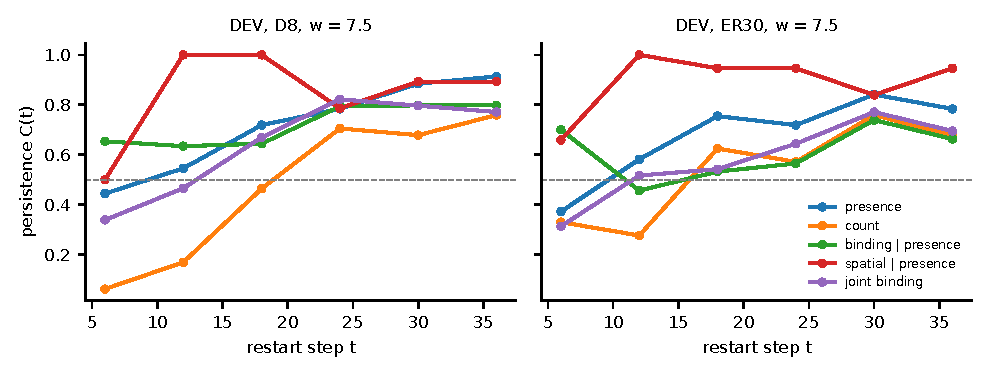
\includegraphics[width=\linewidth]{figures/fig_dev_curves.pdf}
\caption{DEV restart persistence $C(t)$ at $w=7.5$ for the fixed-jump (D8) and equal-ratio (ER30) probes (corrected estimator; exploratory). Dashed line: $C=0.5$.}\label{fig:devcurves}\end{figure}
\begin{table}[t]\centering\small
\caption{DEV persistence steps $t_{50}$ at $w=7.5$ (EXPLORATORY; 163 scenes). $^{\dagger}$left-censored: already above 0.5 at the first grid step.}\label{tab:dev-t50}
\begin{tabular}{lrr}
\toprule
Kind & D8 & ER30 \\
\midrule
presence & 9.3 & 9.7 \\
count & 18.9 & 15.8 \\
binding $\mid$ presence & 6.0$^{\dagger}$ & 6.0$^{\dagger}$ \\
spatial $\mid$ presence & 6.0 & 6.0$^{\dagger}$ \\
joint binding & 13.0 & 11.5 \\
$\Delta t_{50}$ (binding $-$ presence) & -3.29 [-7.56, 8.32] & -3.66 [-6.83, 6.77] \\
\bottomrule
\end{tabular}
\end{table}


\paragraph{Gates.} Table~\ref{tab:dev-gates} lists every pre-declared DEV gate. The HA precision gate failed (half-width \haHalfwidth{} steps against a limit of 4), so HA is exploratory on the test split by the pre-declared rule. The full-resample control failed (maximum $|C|=\fullMaxC$ against $0.15$): the statistic is a maximum over 30 cells, several resting on fewer than ten scenes, so even exactly independent outcomes rarely meet it at this sample size; but presence, the best-supported cell, shows a consistent offset of about $+0.16$ that sampling error does not explain and for which no cause was found in the code. We report it as an open validity concern for the restart estimator. Both HD presence gates passed (\hdPresTwo{} and \hdPresFifteen{} scenes).
\begin{table}[t]\centering\small
\caption{DEV gates (corrected estimator). Failed gates are reported as failed; HA is therefore exploratory.}\label{tab:dev-gates}
\begin{tabular}{llrl}
\toprule
Gate & Criterion & DEV value & Result \\
\midrule
HA precision & CI half-width $\le 4$ steps & 7.94 & failed \\
Full-resample control & $\max|C| \le 0.15$ & 0.57 & failed \\
HD presence, $w=2$ & $\ge 40$ scenes & 45 & passed \\
HD presence, $w=15$ & $\ge 40$ scenes & 59 & passed \\
CAG quality (HPS v2), $w_{lo}=1$ & mean drop $\le 0.5$ & -0.52 & failed \\
CAG quality (HPS v2), $w_{lo}=3$ & mean drop $\le 0.5$ & -0.26 & passed \\
\bottomrule
\end{tabular}
\end{table}


\paragraph{CAG quality guard.} HPS~v2 scored the \hpsPairs{} DEV guard images per $w_{lo}$ against their constant-CFG partners (same prompt and seed). With $w_{lo}=1$ the mean change was \hpsOne{} HPS points (95\% interval \hpsOneLo{} to \hpsOneHi), a drop just beyond the pre-declared $0.5$; with $w_{lo}=3$ it was \hpsThree{} (\hpsThreeLo{} to \hpsThreeHi). By the pre-declared rule $w_{lo}=3$ was adopted before the test split (Figure~\ref{fig:hps}). The switch steps derived from DEV are $s^\star=12$ for prompts whose latest type is presence, binding or spatial relation and $s^\star=21$ for prompts with counts (global $s^\star=\sStarGlobal$).
\begin{figure}[t]\centering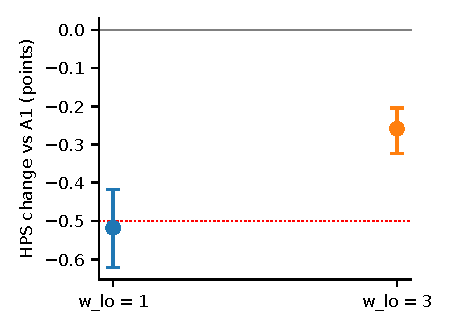
\includegraphics[width=0.45\linewidth]{figures/fig_hps_guard.pdf}
\caption{DEV CAG quality guard: mean HPS~v2 change of CAG images relative to constant CFG~7.5 (95\% scene-bootstrap intervals). Dotted line: pre-declared limit $-0.5$.}\label{fig:hps}\end{figure}

\section{Results: HA (constraint-specific persistence)}\label{sec:resHA}
HA is exploratory: its DEV precision gate failed (Section~\ref{sec:resDEV}). \pending{TEST restart branches have not been generated; TEST is sealed}.
\begin{table}[t]
\centering\small
\caption{Confirmatory results (placeholder).}
\label{tab:results-pending}
\begin{tabular}{ll}
\toprule
Result & Status \\
\midrule
HA: $\Delta t_{50}$ with 95\% CI & PENDING \\
HD: $t_{50}(15)-t_{50}(2)$ & PENDING \\
HE: $\Delta F$, $\Delta$ diversity, CAG minus reversed & PENDING \\
HF: ordering concordance, within-type Spearman & PENDING \\
\bottomrule
\end{tabular}
\end{table}


\section{Results: HD (CFG and persistence)}\label{sec:resHD}
\pending{requires TEST branches at CFG 2, 7.5 and 15 and the frozen protocol}. In the pilot, outcomes of the same prompt and seed agreed more between CFG 7.5 and 15 than between 2 and 7.5, which motivates HD without testing it.

\section{Results: HF and HE}\label{sec:resHFHE}
\textbf{HF} \pending{requires TEST attention maps and the HA curves}. \textbf{HE} \pending{requires DEV-derived switch steps, the CAG quality-guard decision and the TEST arms}. The pilot's global attention re-weighting is not a test of either.

\section{Discussion}\label{sec:discussion}
\paragraph{What CFG changes.} The clearest result is a dose--response one. Raising $w$ from 2 to 15 makes object presence persistent earlier: under a restart that re-noises by eight steps, a trajectory at $w=15$ has settled whether its objects appear several steps before a trajectory at $w=2$ (Section~\ref{sec:resROBUST}). Over the same range, the rate at which the objects appear at all rises and saturates near $w\approx10$. Two common worries do not explain the timing effect. Stronger guidance is known to reduce seed diversity, which would raise agreement between any two images. But chance agreement is computed separately at each $w$, is not higher at $w=15$ on these scenes, and the uncorrected agreement shows the same ordering. The worry that does survive is measurement noise. Correcting $C(t)$ for a judge that errs independently on 14\% of images, the audited rate, removes the difference, so the result is informative only to the extent that the presence judge's errors are content-dependent. Our audit measured how often the judge errs, not how its errors are distributed across seeds. Auditing seed-paired images, which would measure that directly, is the most useful next step for this line of work.

\paragraph{Commitment times are not yet a stable property.} The development split suggested an appealing story: colour assignment is fixed at least as early as object presence and numerosity stays open longest. The available test scenes do not reproduce it. Binding becomes persistent after presence, joint binding about eight steps later than on DEV, and the shift appears under both restart probes. Several factors could produce it, and the partial test cannot separate them: a different scene composition, the DEV precision gate that already failed, the unvalidated binding judge, and the left-censoring of the DEV binding curve at the first grid step. We draw one methodological conclusion: a commitment time estimated on about 100 scenes, with intervals of more than $\pm$7 steps, is too imprecise to schedule an intervention on.

\paragraph{Why CAG does not help, and what the controls show.} CAG was meant to spend guidance while a constraint is still open and to release it afterwards. Two findings explain why it did not work here. First, its switch steps came from DEV commitment times that did not transfer, so on the test scenes it lowers guidance at step 12 while binding is still unsettled. Second, its registered comparison confounds timing with dose. Every CAG arm applies less mean guidance than constant $w=7.5$, and the dose-matched controls attribute the diversity gain entirely to that lower mean: the constant schedule at the same mean is as diverse, and the reversed schedule more so. At equal mean, front-loading guidance is the \emph{least} diverse of the three orders and no better in adherence. This agrees with interval guidance \citep{kynkaanniemi2024interval}, which reports that guidance at the highest noise levels harms diversity, and with step-selection results \citep{grimal2025step}, where strengthening the conditioning late helps alignment more than doing so early. Our data add a controlled, dose-matched comparison on compositional constraints; they do not show that any timed schedule beats constant guidance of the same mean. Online, prompt-dependent schedules \citep{dynamiccfg2025} avoid the transfer problem by measuring during sampling, and they are the natural comparison for a revised CAG.

\paragraph{Attention as a cheap proxy.} The step at which cross-attention maps stop changing orders constraint types almost opposite to persistence (concordance \rbHfConc, $[\rbHfLo,\rbHfHi]$), and within types the scene-level correlations are not distinguishable from zero. On this evidence, attention stabilisation in Stable Diffusion~1.5 is not a substitute for the interventional measurement. This is relevant to methods that read early attention as a forecast of the final image \citep{diffusionprobe2026,guo2024initno}. Their target is image quality or alignment, not the timing of a particular constraint, so our result does not contradict them. It does caution against equating attention that has stopped moving with an outcome that has been decided.

\paragraph{What a reader can take from the null results.} Three negative results are informative because the design anticipated them. The full-resample control and the HA precision gate failed on DEV before any test image existed, which is why HA was demoted to exploratory before it could be over-read. HE has a reversed arm and a matched-mean arm, which is what lets us attribute the diversity effect to dose. And the HD stress test shows how precise a judge must be before timing differences of a few steps become interpretable: with independent errors, even 95\% accuracy leaves the HD interval touching zero.

\section{Limitations and threats to validity}
(1) A single model (SD~1.5) and scheduler; no cross-architecture claim. (2) The judge is detector-based, unaudited on DEV, and the pilot check is non-independent and small. (3) Restart persistence is defined relative to a re-noising magnitude that varies with the step; absolute $\tfifty$ is not a model property. (4) Conditional outcomes select on a generated variable. (5) HA precision may fail its gate with realistic judge noise. (6) Detector and CLIP model revisions are not pinned in code. (7) Hardware-specific identity was tested on few cases. (8) Throughput varies between sessions. (9) The prior-art review is incomplete and novelty is not claimed. (10) Relative size rests on 24 object pairs only. (11) The reversed guidance arm can need very high guidance when the switch step is late. (12) Labels and code were produced with AI assistance; provenance must be disclosed according to the event or venue policy.

\section{Hypothesis roadmap (exploratory; post hoc until separately specified)}
Candidate extensions are ranked by scientific value, novelty uncertainty, feasibility, compute and dependency readiness, and none is confirmatory: (a) first-mentioned-object and mention-order effects on binding under matched seeds; (b) numerosity compression toward three in counting; (c) guidance attribution to constraint tokens; (d) layer-group knockouts with matched random controls; (e) outcome fragility under micro-perturbations; (f) negative-prompt timing for binding repair; (g) a second architecture if tooling and compute allow. The ledger in \texttt{docs/HYPOTHESIS\_LEDGER.md} records each with its status.

\section{Reproducibility and provenance}\label{sec:repro}
All decision rules, development-set constants and test manifests were frozen in a signed protocol before any test image was generated. Every reported number is generated from saved, checksummed outputs by versioned scripts, and generation itself is deterministic given the manifest, so any result can be recomputed without regenerating images. Appendix~\ref{app:repro} lists the generators and the provenance record. Deviations from the registered plan are disclosed where they occur: the chance-agreement correction before the test split (Section~\ref{sec:resDEV}), the single-annotator audit (Section~\ref{sec:evaluation}), and every post-hoc analysis (Sections~\ref{sec:resROBUST} and~\ref{sec:resATTN}).

\section{Conclusion}
We asked when compositional constraints become persistent during diffusion sampling and what classifier-free guidance changes about that timing. On the available two-thirds of a pre-registered test split, stronger guidance makes object presence persistent earlier, and cross-attention shows the same shift: object nouns separate earlier on identical noise, and missed objects are visible as diffuse, overlapping attention from the first steps. Both findings are exploratory. The timing result holds only if the presence judge's errors are not independent across seeds.

The intervention built on the measurement did not work. Commitment times from the development split did not transfer, and Commitment-Aligned Guidance neither kept adherence nor beat its reversed schedule; matched-mean controls showed that its extra diversity came from lower average guidance. The broader lesson is about precision. Guiding by commitment time requires timing estimates far tighter than about 100 scenes provide, and judges that are validated, including for their error structure, for more than object presence. Three steps remain:
\begin{itemize}
\item the registered confirmatory analysis, once the three missing shards exist;
\item a seed-paired judge audit;
\item a 400-image experiment that resolves the full-resample offset.
\end{itemize}

\bibliographystyle{plainnat}
\bibliography{references}
\end{document}
